% Settings for the default beamer theme
\documentclass[english, aspectratio=169]{beamer}
\usepackage[T1]{fontenc}
\usepackage[utf8]{inputenc}
\usepackage{tabularx}
\usepackage{babel}
\usepackage[ruled,vlined]{algorithm2e}
\SetAlgorithmName{Algoritmus}{algoritmus}{List of Algorithms}
\setcounter{secnumdepth}{3}
\setcounter{tocdepth}{3}

\makeatletter

\newcommand\makebeamertitle{\frame{\maketitle}}

% (ERT) argument for the TOC
\AtBeginDocument{%
  \let\origtableofcontents=\tableofcontents
  \def\tableofcontents{\@ifnextchar[{\origtableofcontents}{\gobbletableofcontents}}
  \def\gobbletableofcontents#1{\origtableofcontents}
}

% Theme settings
\usetheme{Frankfurt}
\usecolortheme{default}
\usefonttheme[onlymath]{serif}

% Template settings
\setbeamertemplate{navigation symbols}{}
\setbeamertemplate{blocks}[rounded][shadow=false]
\setbeamertemplate{title page}[default][colsep=-4bp, rounded=true, shadow=false]
\makeatother

% Define a custom darker red color
\definecolor{DarkerRed}{RGB}{139,0,0} % Adjust the RGB values as needed

% Use the newly defined color in Beamer theme elements
\setbeamercolor{structure}{fg=DarkerRed} % Changes basic structural elements to Darker Red
\setbeamercolor{title in head/foot}{bg=DarkerRed} % Changes the title in header/footer to Darker Red


\begin{document}

% Title page
\section{Bevezetés}
\title[]{Üzleti Elemzések Módszertana}
\subtitle{9. Előadás: Ajánló rendszerek}
\author[Kuknyó Dániel]{Kuknyó Dániel\\Budapesti Gazdasági Egyetem}
\date{2023/24\\2.félév}
\makebeamertitle

% Table of contents slide
\begin{frame}
\tableofcontents{}
\end{frame}

% Table of contents of the current section
\begin{frame}
\tableofcontents[currentsection]
\end{frame}

\begin{frame}{Hosszú farok eloszlás}
\begin{columns}
\begin{column}{.5\textwidth}
A webes vásárlás elterjedése előtt az volt a jellemző, hogy kevés termék generálta a forgalom legnagyobb hányadát. Mivel az üzlethelyiségben a férőhely limitált volt, a kevesek által keresett termékek nem kaptak helyet a polcon.\par\medskip
Az internetes kereskedelem elterjedése helyet adott az ún. \emph{niche}, vagyis szűk csoportok számára népszerű termékeknek, amelyek specifikus felhasználásukkal vonzzák be a célközönséget
\end{column}
\begin{column}{.5\textwidth}
\begin{center}
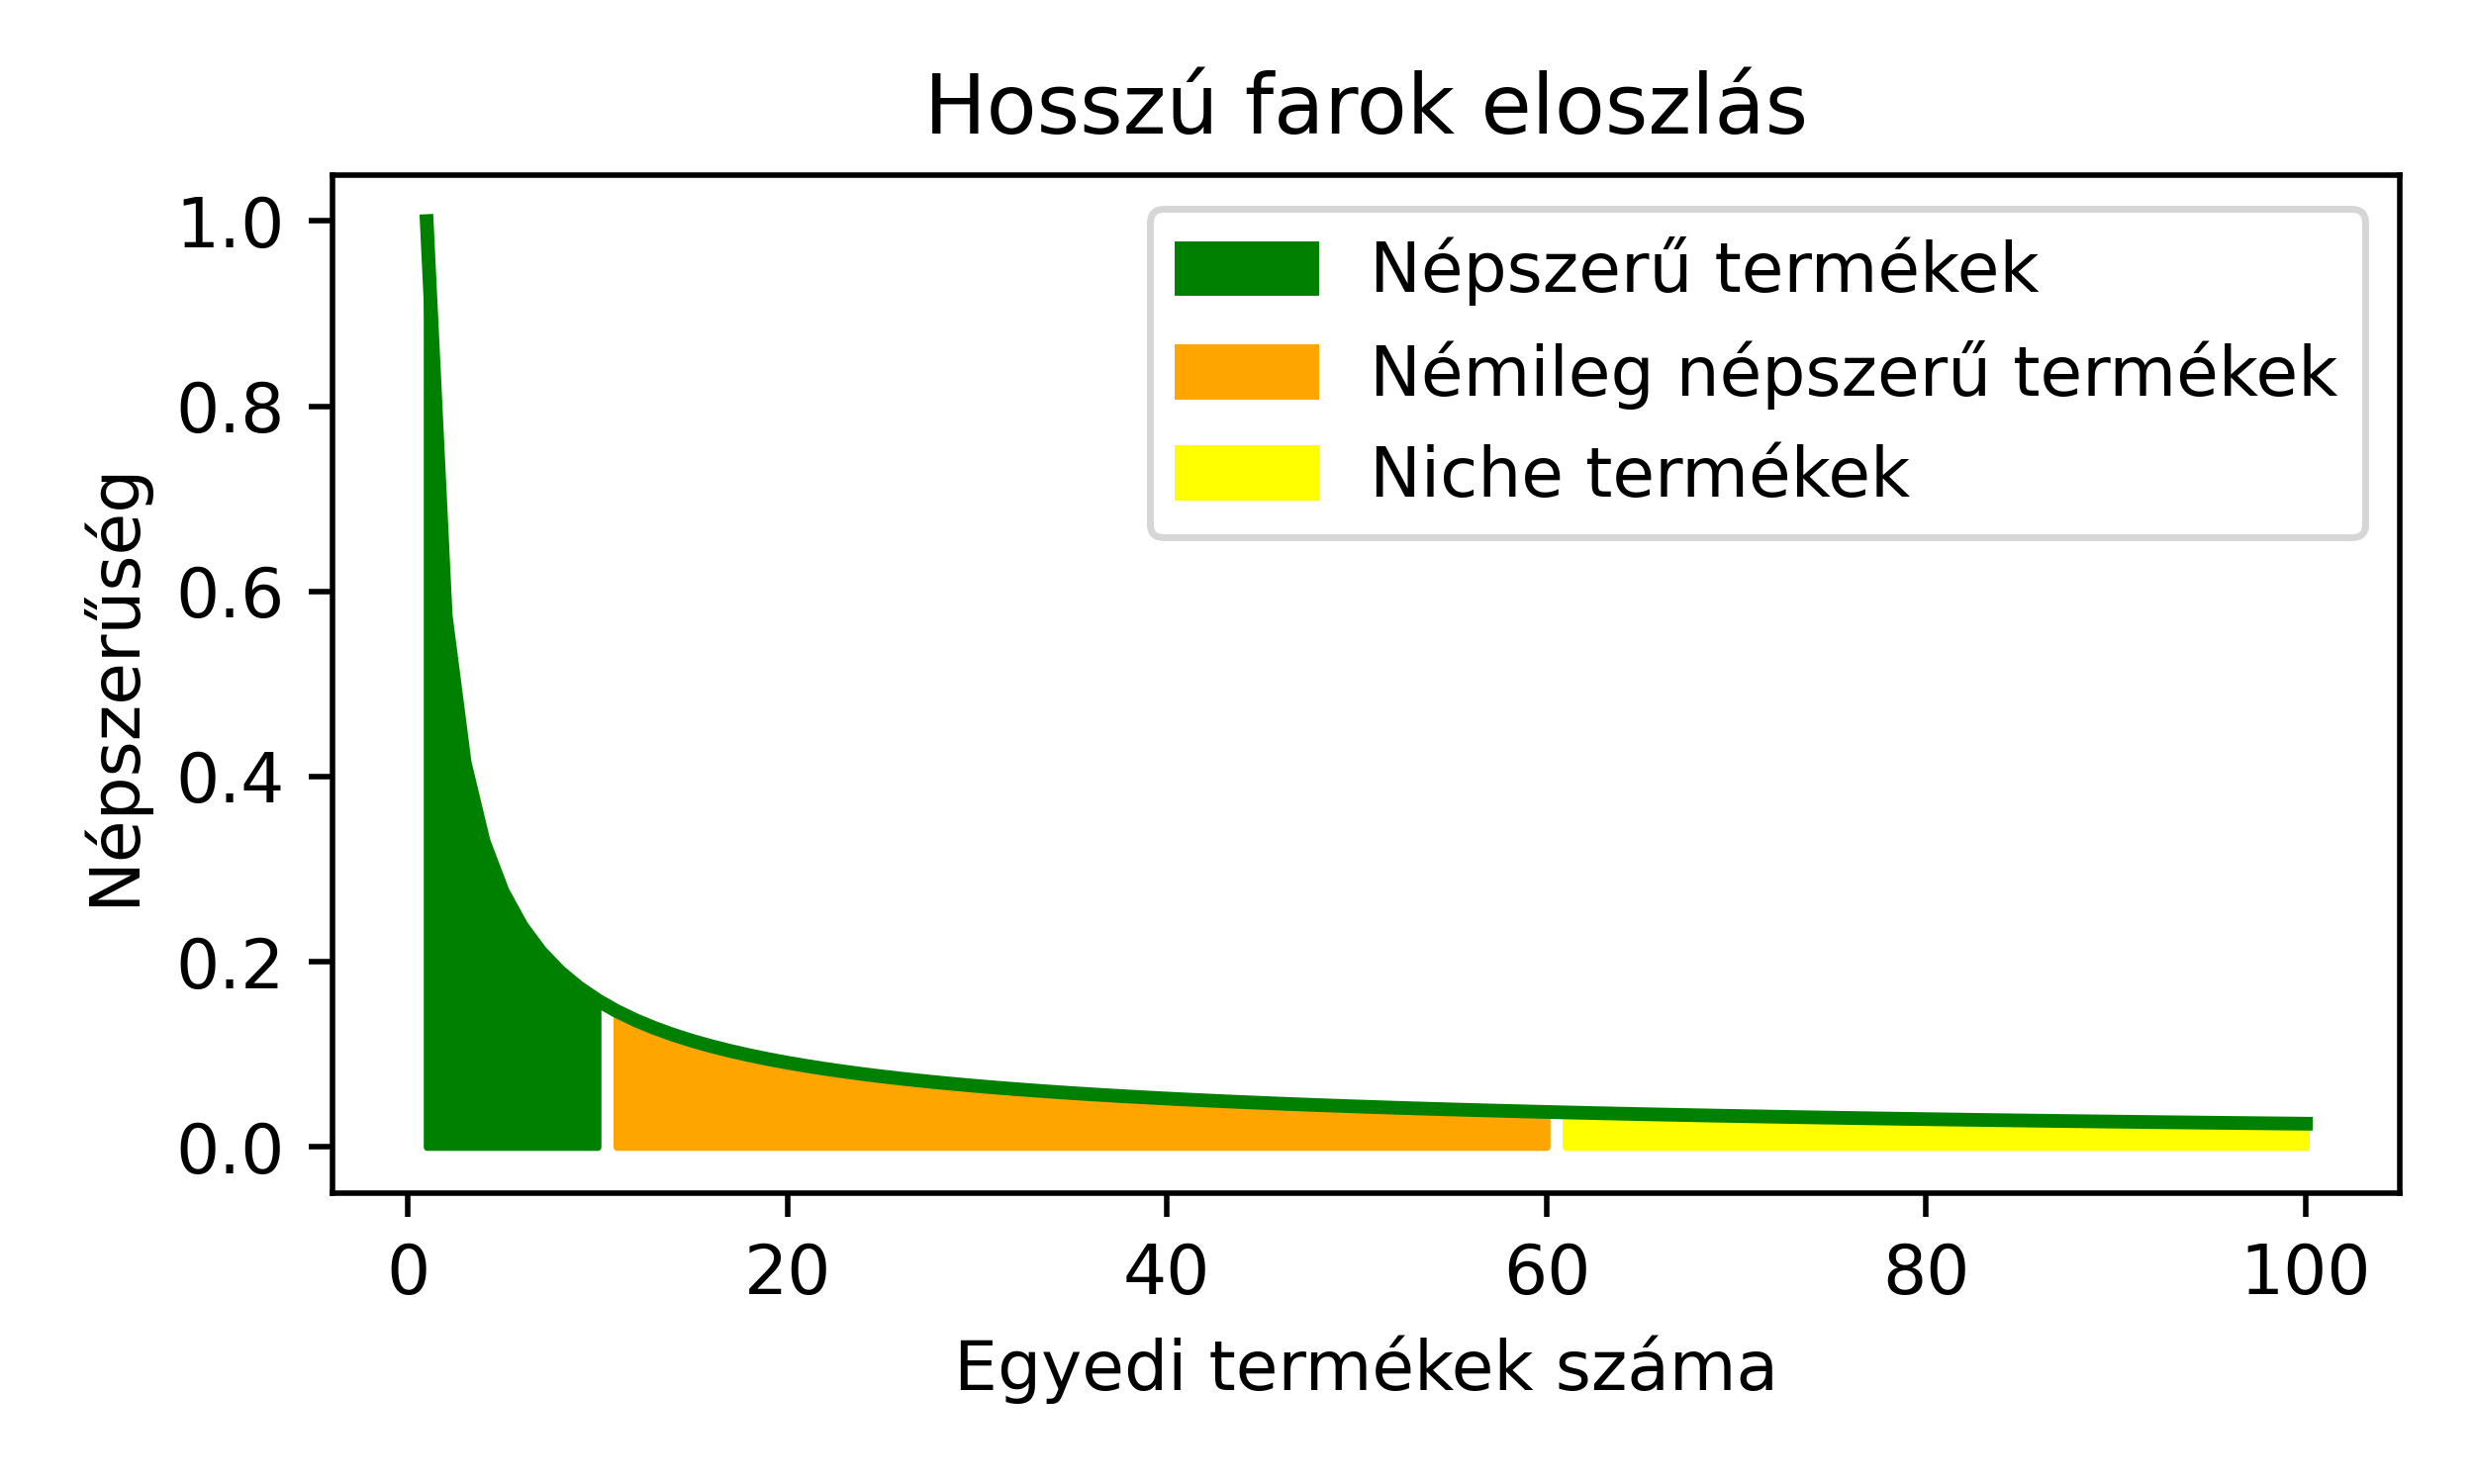
\includegraphics[width=7cm, height=7cm, keepaspectratio]{images/recommender_1.png}
\end{center}
\end{column}
\end{columns}
\end{frame}

\begin{frame}{Ajánló rendszerek}
\begin{columns}
\begin{column}{.5\textwidth}
Olyan technikák vagy rendszerek, \textbf{amelyek valamilyen terméket, szolgáltatást vagy entitást kötnek össze más termékekkel, javaslatokkal vagy entitásokkal a rendelkezésükre álló információ alapján}.\par\smallskip
Az ajánló rendszerek célja objektumok közötti leképezések felderítése, mint: 
\begin{itemize}
	\item Filmek
	\item Termékek
	\item Könyvek
	\item Média
\end{itemize}
\end{column}
\begin{column}{.5\textwidth}
\begin{center}
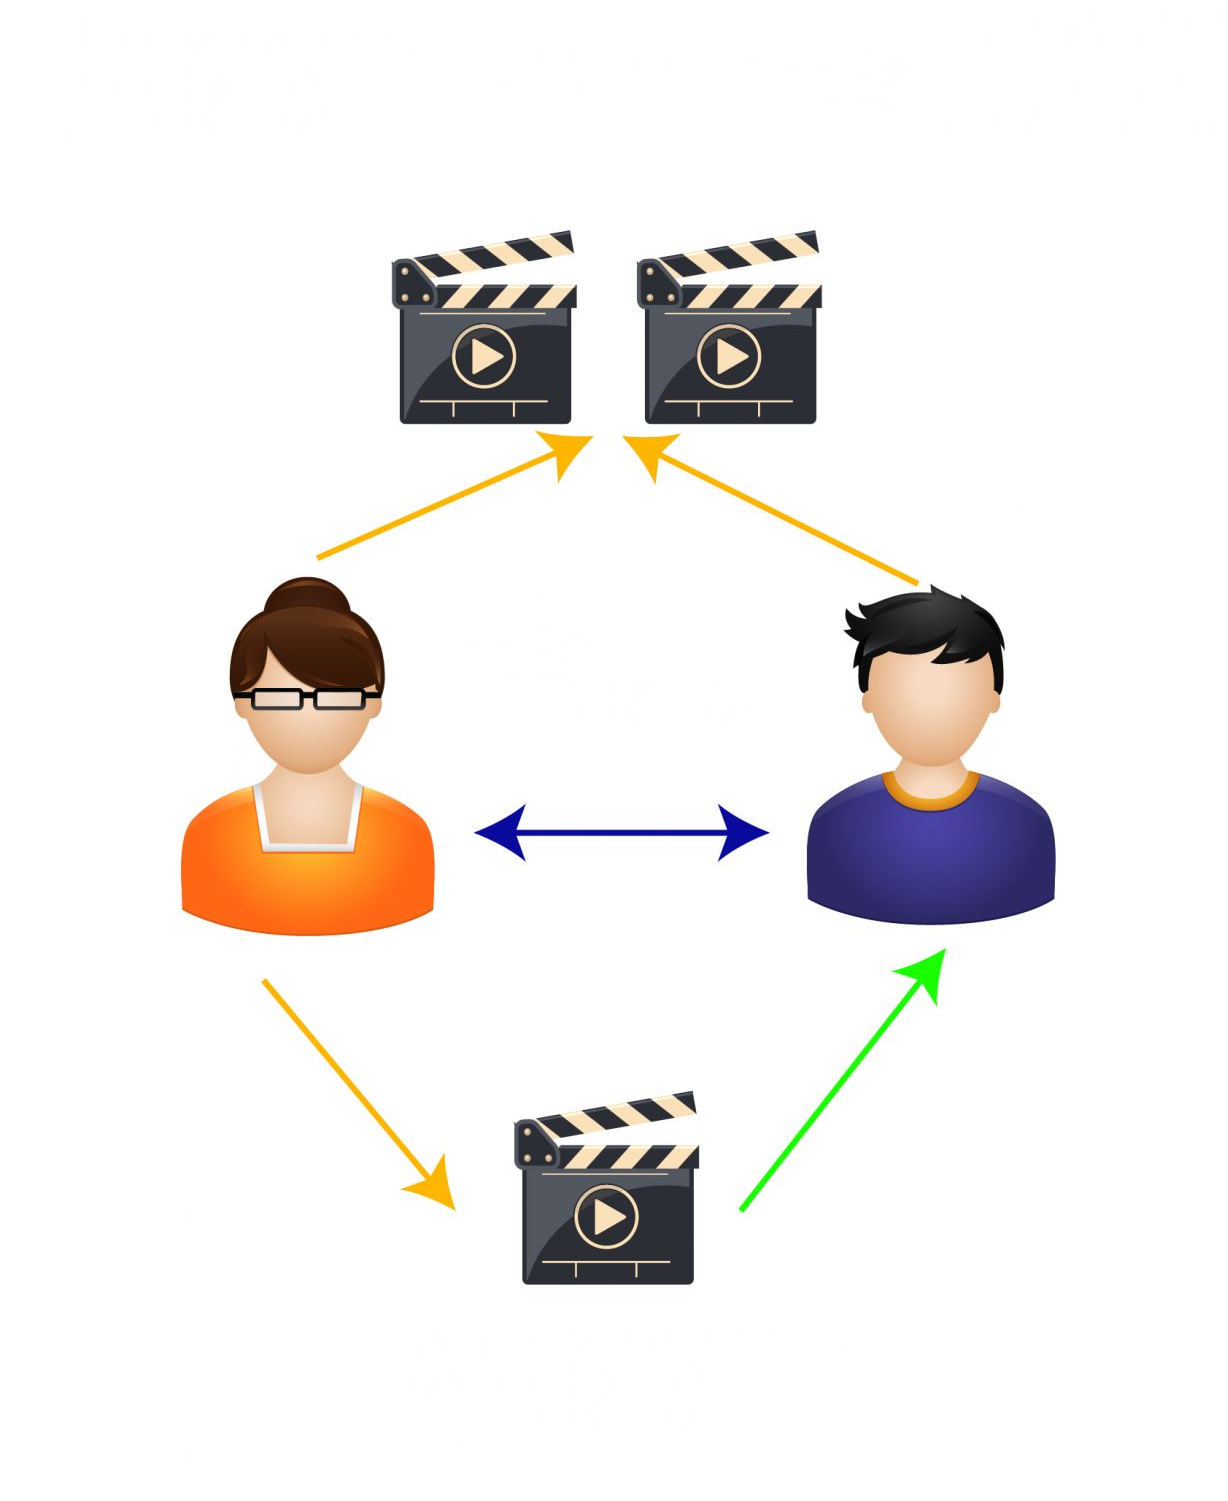
\includegraphics[width=7cm, height=7cm, keepaspectratio]{images/recommender_2.png}
\end{center}
\end{column}
\end{columns}
\end{frame}

\begin{frame}{Ajánlat előállításának szintjei}
\begin{columns}
\begin{column}{.4\textwidth}
A rendszer célja, hogy ajánlásokat tegyen a rendelkezésre álló információ alapján.\par\medskip
Különböző rendszertípusoknak különböző igénye van az adatok forrásával, milyenségével és rendelkezésre állásával szemben.\par\medskip
A rendszereket lehetséges célnak megfelelően optimalizálni a népszerűség vagy személyre szabottságnak megfelelően.
\end{column}
\begin{column}{.6\textwidth}
\begin{center}
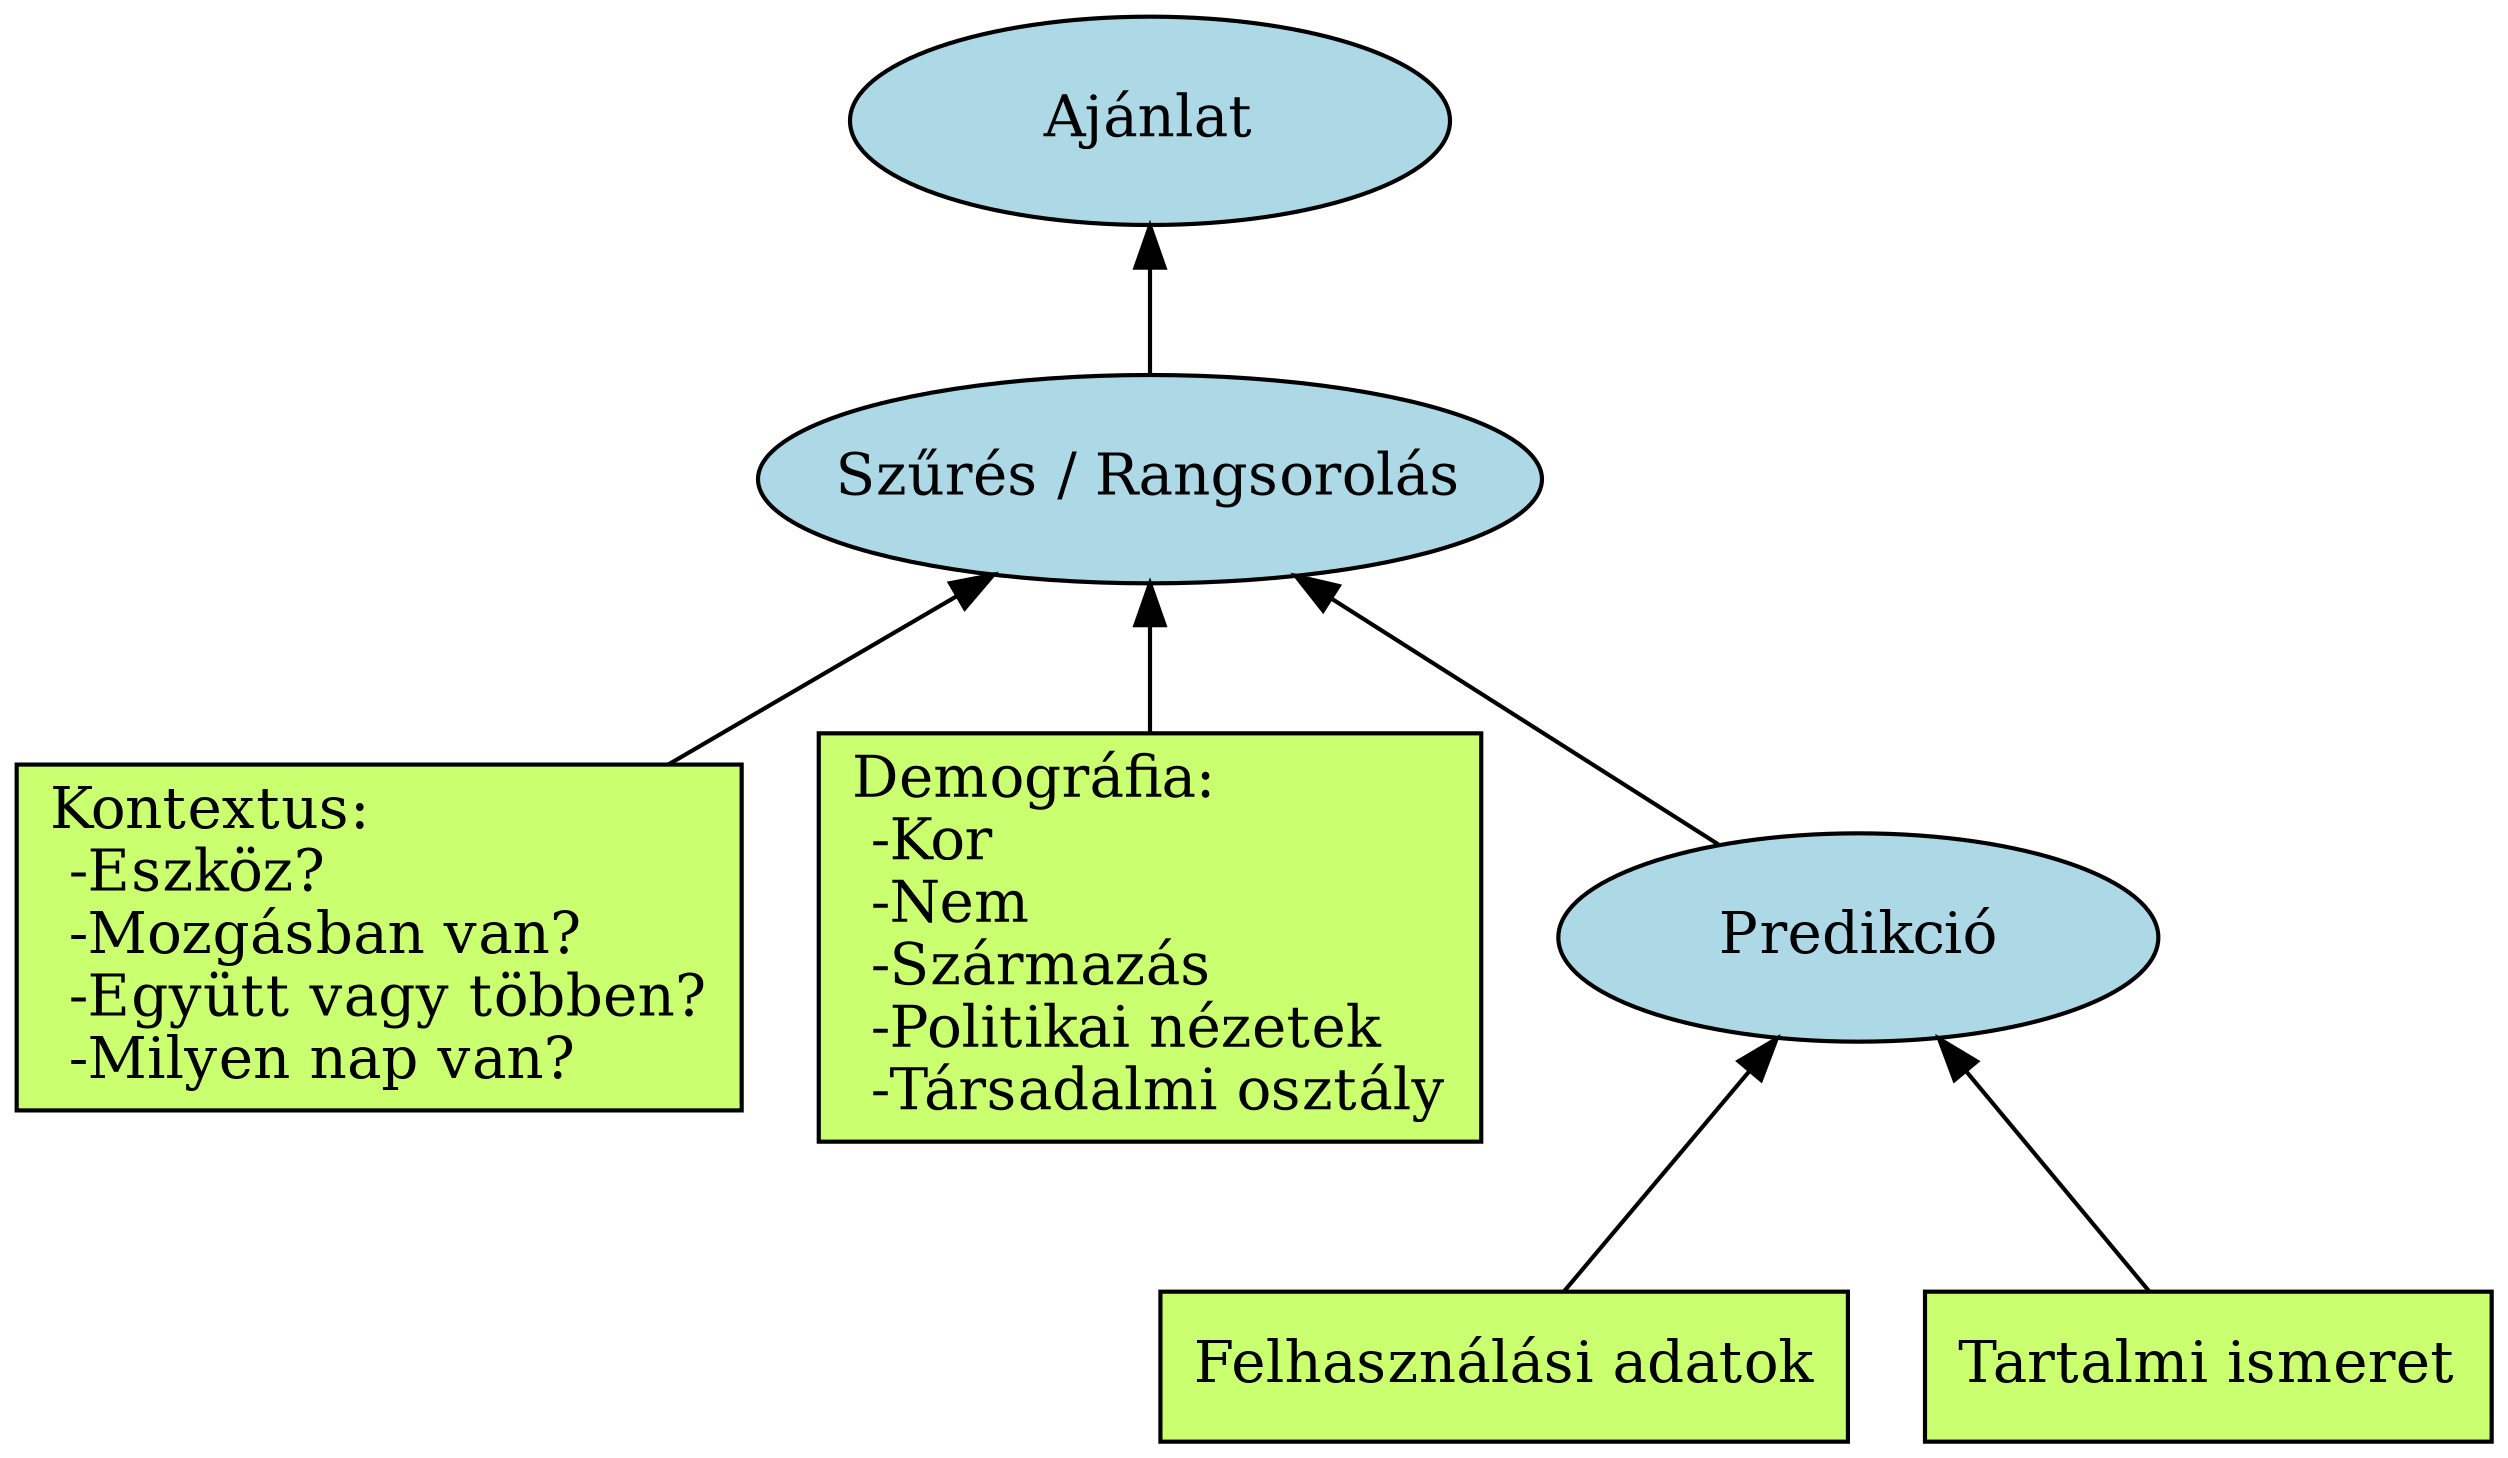
\includegraphics[width=8cm, height=7cm, keepaspectratio]{graphs/recommender_1.png}
\end{center}
\end{column}
\end{columns}
\end{frame}

\begin{frame}{Ajánlatok személyre szabottsága}
\begin{columns}
\begin{column}{.5\textwidth}
Egy ajánló rendszer által adott ajánlat a személyre szabottól a népszerűig terjedhet.\par\medskip
A személyre szabott ajánlatok a felhasználó egyedi igényét célozzák, és ezért több felhasználási adatot igényelnek.\par\medskip
A népszerűségen alapuló ajánlatoknak nincs szüksége felhasználási adatokra, de nem képes az egyén ízlésének megfelelő ajánlatot előállítani.
\end{column}
\begin{column}{.5\textwidth}
\begin{center}
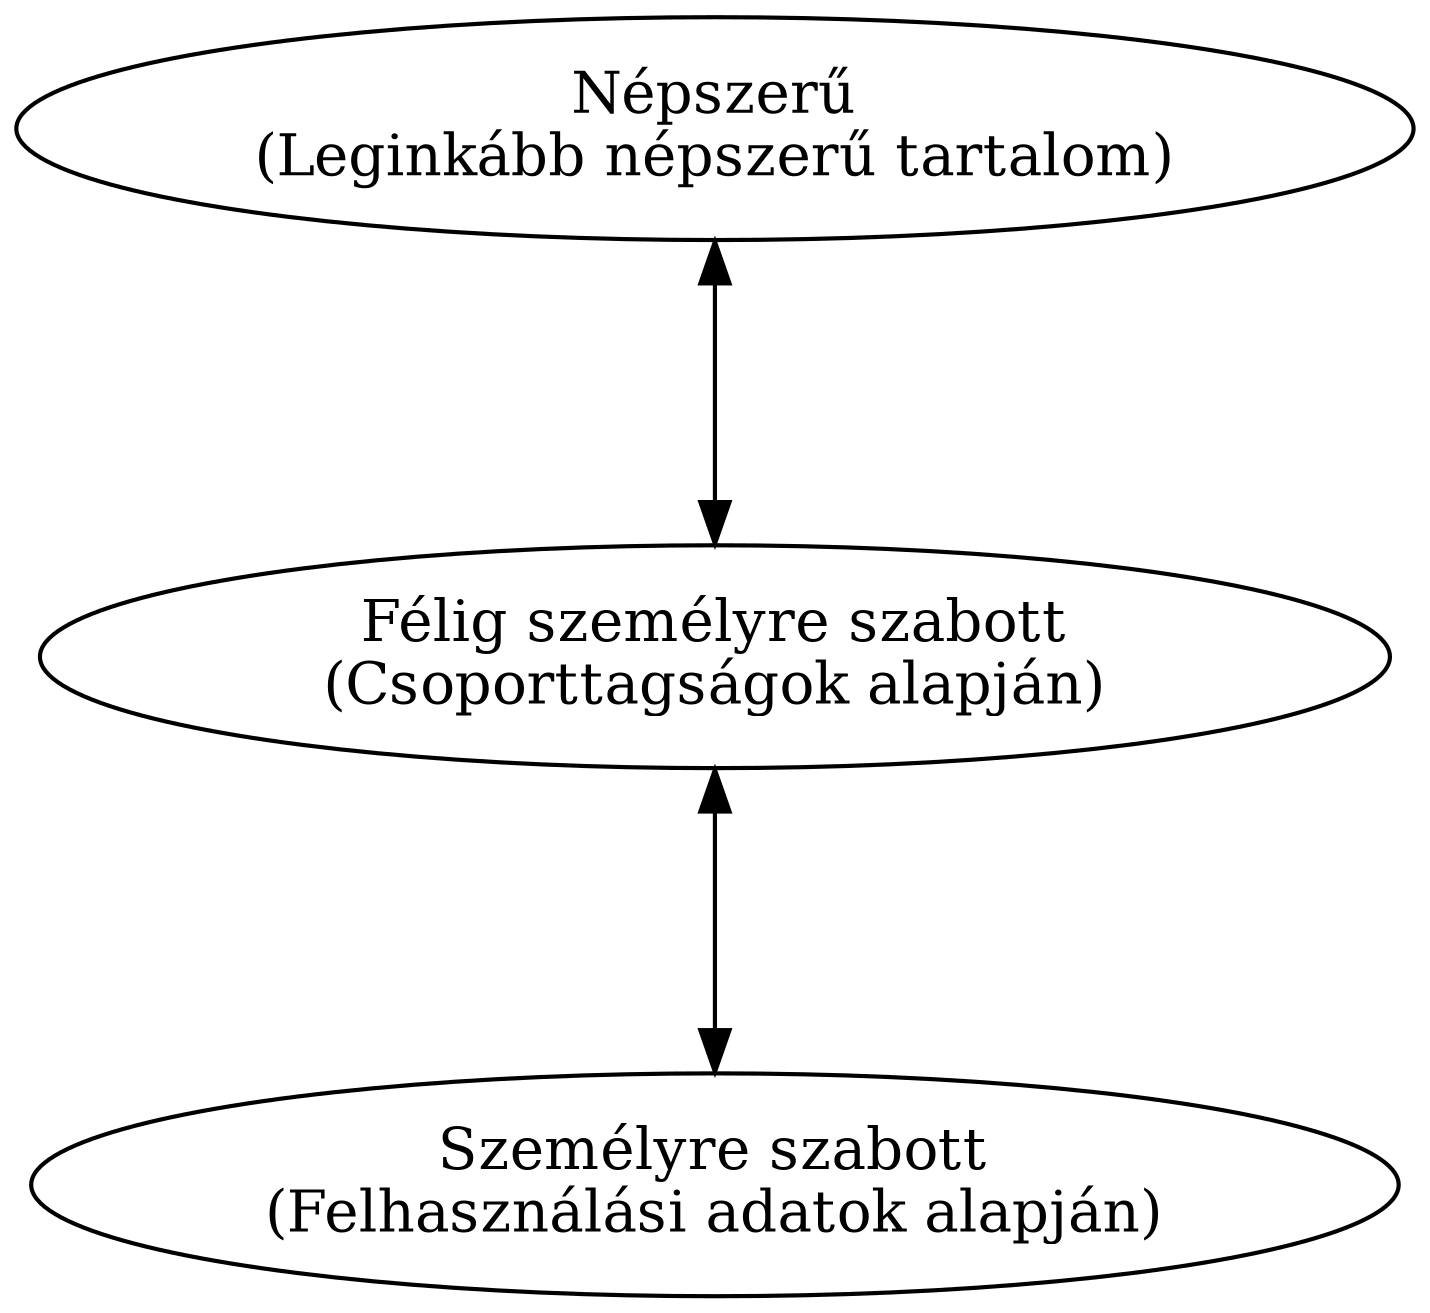
\includegraphics[width=7cm, height=7cm, keepaspectratio]{graphs/recommender_2.png}
\end{center}
\end{column}
\end{columns}
\end{frame}

\begin{frame}{A predikciós probléma}
\begin{columns}
\begin{column}{.5\textwidth}
Adott egy $m$ felhasználóból és $n$ termékből álló $X$ mátrix. $X\left[ u,i \right]$ azt jelöli, hogy $u$ felhasználó hogyan értékelte $i$ terméket.\par\medskip
A feladat megbecsülni a mátrix hiányzó értékeit a termékekről és felhasználókról rendelkezésre álló információ alapján.\par\medskip
Ez a mátrix leggyakrabban egy ritka mátrix: nagyon sok az ismeretlen érték.
\end{column}
\begin{column}{.5\textwidth}
\begin{center}
\begin{tabular}{|c|c|c|c|c|c|c|}
\hline
& $i_1$ & $i_2$ & $i_3$ & $i_4$ & $i_5$ & $i_6$ \\
\hline
$u_1$ & $4$ & $?$ & $3$ & $?$ & $5$ & $?$ \\
\hline
$u_2$ & $?$ & $2$ & $?$ & $?$ & $4$ & $1$ \\
\hline
$u_3$ & $?$ & $?$ & $1$ & $?$ & $2$ & $5$ \\
\hline
$u_4$ & $?$ & $?$ & $3$ & $?$ & $?$ & $1$ \\
\hline
$u_5$ & $1$ & $4$ & $?$ & $?$ & $2$ & $5$ \\
\hline
$u_6$ & $5$ & $?$ & $2$ & $1$ & $?$ & $4$ \\
\hline
$u_7$ & $?$ & $2$ & $3$ & $?$ & $4$ & $5$ \\
\hline
\end{tabular}
\end{center}
\end{column}
\end{columns}
\end{frame}

\begin{frame}{A rangsorolási probléma}
\begin{columns}
\begin{column}{.5\textwidth}
A rangsorolási probléma a predikciós problémának egy intuitívabb megfogalmazása.\par\smallskip
Ha adott $n$ elem halmaza, a rangsorolás célja megkülönböztetni a leginkább javasolható $k$ elemet, amit ajánlhat a felhasználónak valamilyen rendezési kritérium alapján.\par\smallskip
A predikciós probléma gyakran rangsorolási problémához vezet vissza.
\end{column}
\begin{column}{.5\textwidth}
\begin{center}
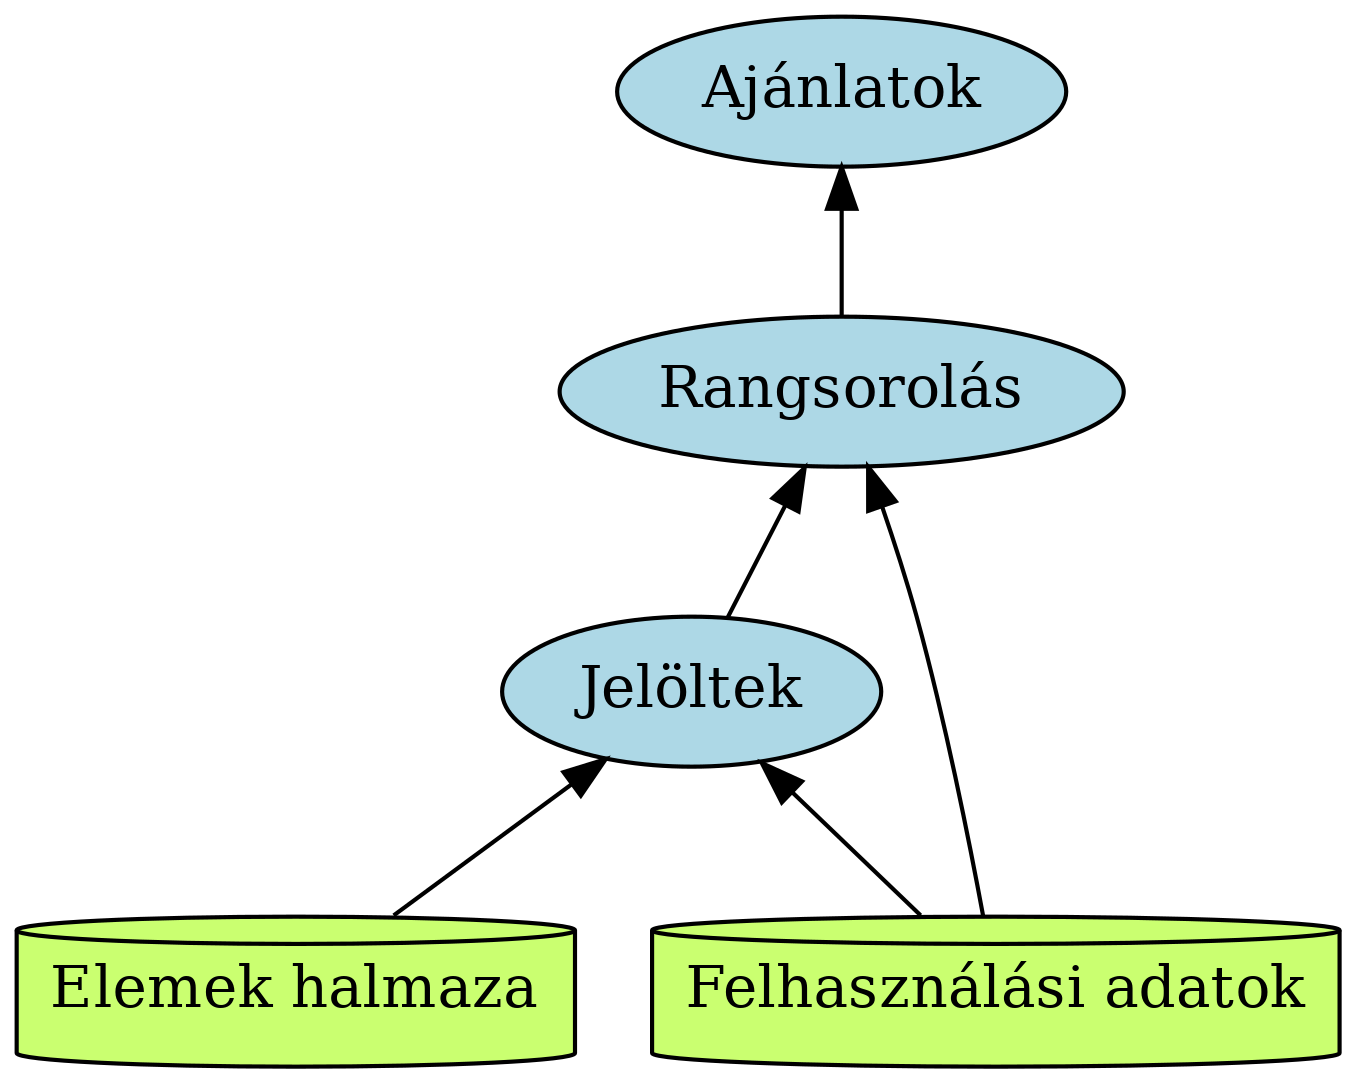
\includegraphics[width=7cm, height=7cm, keepaspectratio]{graphs/recommender_3.png}
\end{center}
\end{column}
\end{columns}
\end{frame}

\section{Kollaboratív szűrők}

\begin{frame}
\tableofcontents[currentsection]
\end{frame}

\begin{frame}{Kollaboratív szűrők}
\begin{columns}
\begin{column}{.5\textwidth}
\begin{block}{Kollaboratív szűrő}
Olyan ajánló rendszer, amely a közösség által adott értékelésekből, felhasználási metrikákból állít össze javaslatokat.
\end{block}
Két típusa létezik:
\begin{itemize}
	\item \textbf{Felhasználó alapú}: Az adott felhasználónak a hozzá hasonló felhasználók preferenciái alapján ajánl termékeket.
	\item \textbf{Termék alapú}: Olyan elemeket ajánl a felhasználónak, amelyek hasonlóak az általa preferált elemekhez.
\end{itemize}
\end{column}
\begin{column}{.5\textwidth}
\begin{center}
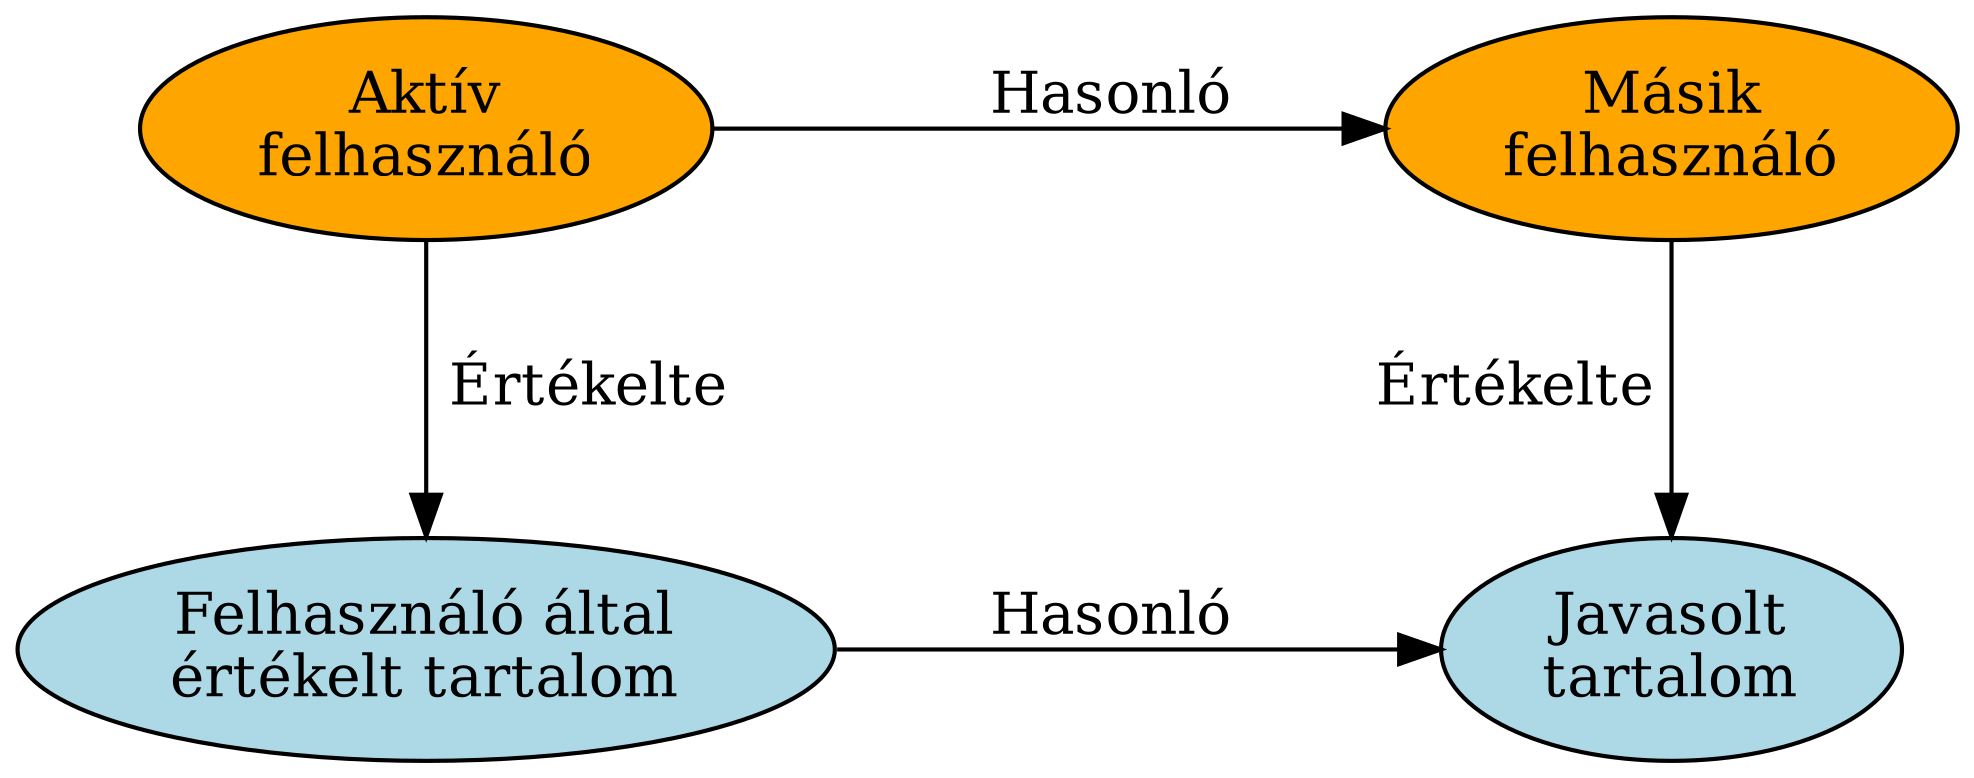
\includegraphics[width=7cm, height=7cm, keepaspectratio]{graphs/recommender_4.png}
\end{center}
\end{column}
\end{columns}
\end{frame}

\begin{frame}{Termék alapú kollaboratív szűrő eljárása}
A példában a cél $u_1$ felhasználó értékelésének megbecsülése az AV filmhez. Ehhez tartozóan  az eljárás először kiszámítja az AV film hasonlóságát az összes többivel, majd ezeket rangsorolja és a leghasonlóbb elemek értékelései alapján megadja annak becsült értékelését.\par\medskip
\begin{center}
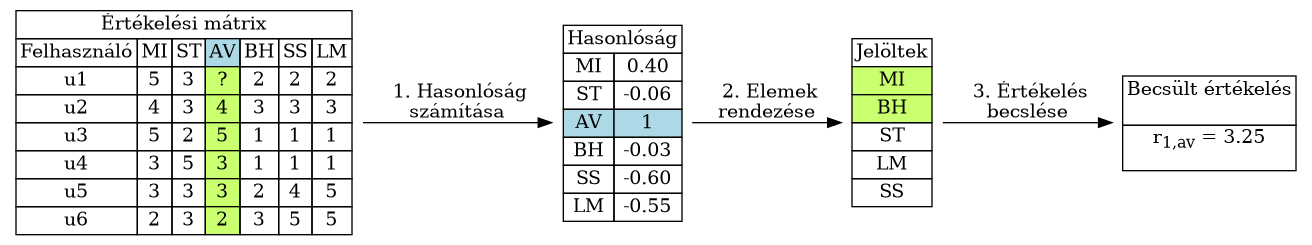
\includegraphics[width=14cm, height=7cm, keepaspectratio]{graphs/recommender_5.png}
\end{center}
\end{frame}

\begin{frame}{Két egyed hasonlóságának kiszámítása}
\begin{columns}
\begin{column}{.5\textwidth}
\begin{block}{Elemek hasonlósága}
\[
sim\left( i_1,i_2 \right) = \frac{\sum_u\left( nr_{i_1,u} \cdot nr_{i_2,u} \right)}{\sqrt{\sum_u nr^2_{i_1,u}} \cdot \sqrt{\sum_u nr^2_{i_1,u}}}
\]
Ahol:
\begin{itemize}
	\item $r_{i,u}$: $u$ felhasználó értékelése $i$ elemre
	\item $\bar{r}_u$: $u$ felhasználó átlagos értékelése
	\item $nr_{i,u}=r_{i,u} - \bar{r}_u$: Normalizálási tényező
\end{itemize}
\end{block}
\end{column}
\begin{column}{.5\textwidth}
\begin{block}{Felhasználók hasonlósága}
\[
\text{sim}(u_1, u_2) = \frac{\sum_{i} (nr_{i,u_1} \cdot nr_{i,u_2})}
{\sqrt{\sum_{i} (nr_{i,u_1})^2} \cdot \sqrt{\sum_{i} (nr_{i,u_2})^2}}
\]
Ahol:
\begin{itemize}
    \item \( r_{i,u} \): $u$ felhasználó értékelése $i$ elemre
    \item \( \bar{r}_u \): az u felhasználó átlagos értékelése
    \item \( nr_{i,u} = r_{i,u} - \bar{r}_u \): az értékelések normalizálása, a felhasználó átlagától való eltérés
\end{itemize}
\end{block}
\end{column}
\end{columns}
\end{frame}

\begin{frame}{Hasonlóság kiszámítása minden mintaegyedre}
Az ajánlásokhoz érdemes a hasonlóságokat előzetesen kiszámolni, hogy csökkentse a teljes rendszer erőforrásigényét. Ehhez tartozóan a hasonlósági mátrix létrehozásának algoritmusa:
\begin{algorithm}[H]
\caption{Termék-termék kollaboratív szűrő}
\SetAlgoLined
	\For{Termék $i_1$ a katalógusban}{
		\For{Felhasználó $u$ aki fogyasztotta $i_1$ terméket}{
			\For{Termék $i_2$ amit $u$ fogyasztott}{
				Termékpáros $\left( i_1,i_2 \right)$ rögzítése
			}
			\For{Minden $i_2$ termékre}{
				$sim\left( i_1, i_2 \right)$ kiszámítása
			}
		}
	}
\end{algorithm}
\end{frame}

\begin{frame}{Példa: hasonlósági tábla összeállítása}
Adott az alábbi értékelési mátrix 6 filmmel és 6 felhasználóval. A cél megbecsülni a táblázat hiányzó értékeit. Első lépésben el kell menteni, melyik filmeket látták még azok a felhasználók, amelyek egy adott filmet megnéztek:
\begin{columns}
\begin{column}{.3\textwidth}
\begin{small}
\vspace{.5cm}\\
$MIB: \left[ ST,B,SS,LM,AV \right]$\\
$ST: \left[ MIB, B, SS, LM, AV \right]$\\
$B: \left[ MIB, ST, SS, LM, AV \right]$\\
$SS: \left[ MIB, ST, B, LM, AV \right]$\\
$LM: \left[ MIB, ST, SS, B, AV \right]$\\
$AV: \left[ MIB, ST, B, SS, LM \right]$\\
\end{small}
\end{column}
\begin{column}{.8\textwidth}
\begin{center}
\begin{footnotesize}
\begin{tabular}{|c|c|c|c|c|c|c|}
\hline
& 

\includegraphics[height=1.5cm, keepaspectratio]{images/movies/men_in_black.png} &
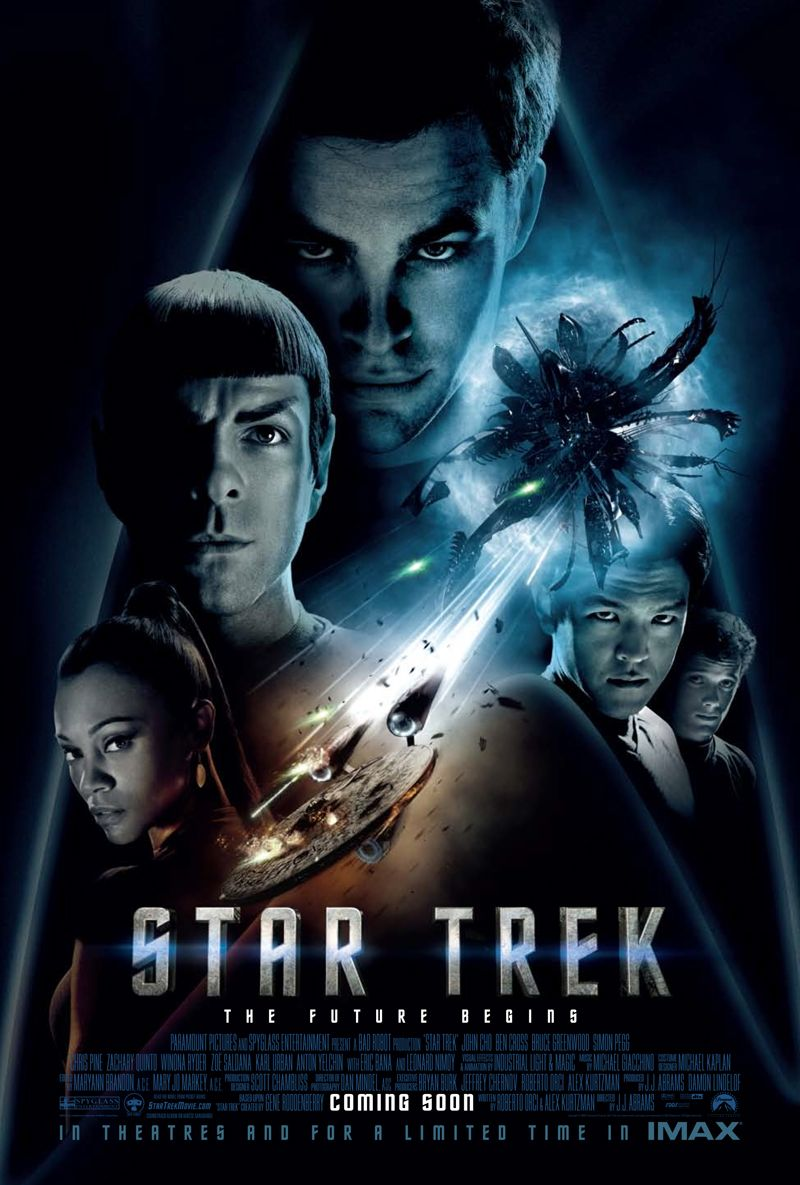
\includegraphics[height=1.5cm, keepaspectratio]{images/movies/star_trek.png} &

\includegraphics[height=1.5cm, keepaspectratio]{images/movies/ace_ventura.png} &

\includegraphics[height=1.5cm, keepaspectratio]{images/movies/braveheart.png} &

\includegraphics[height=1.5cm, keepaspectratio]{images/movies/sense_and_sensibility.png} &
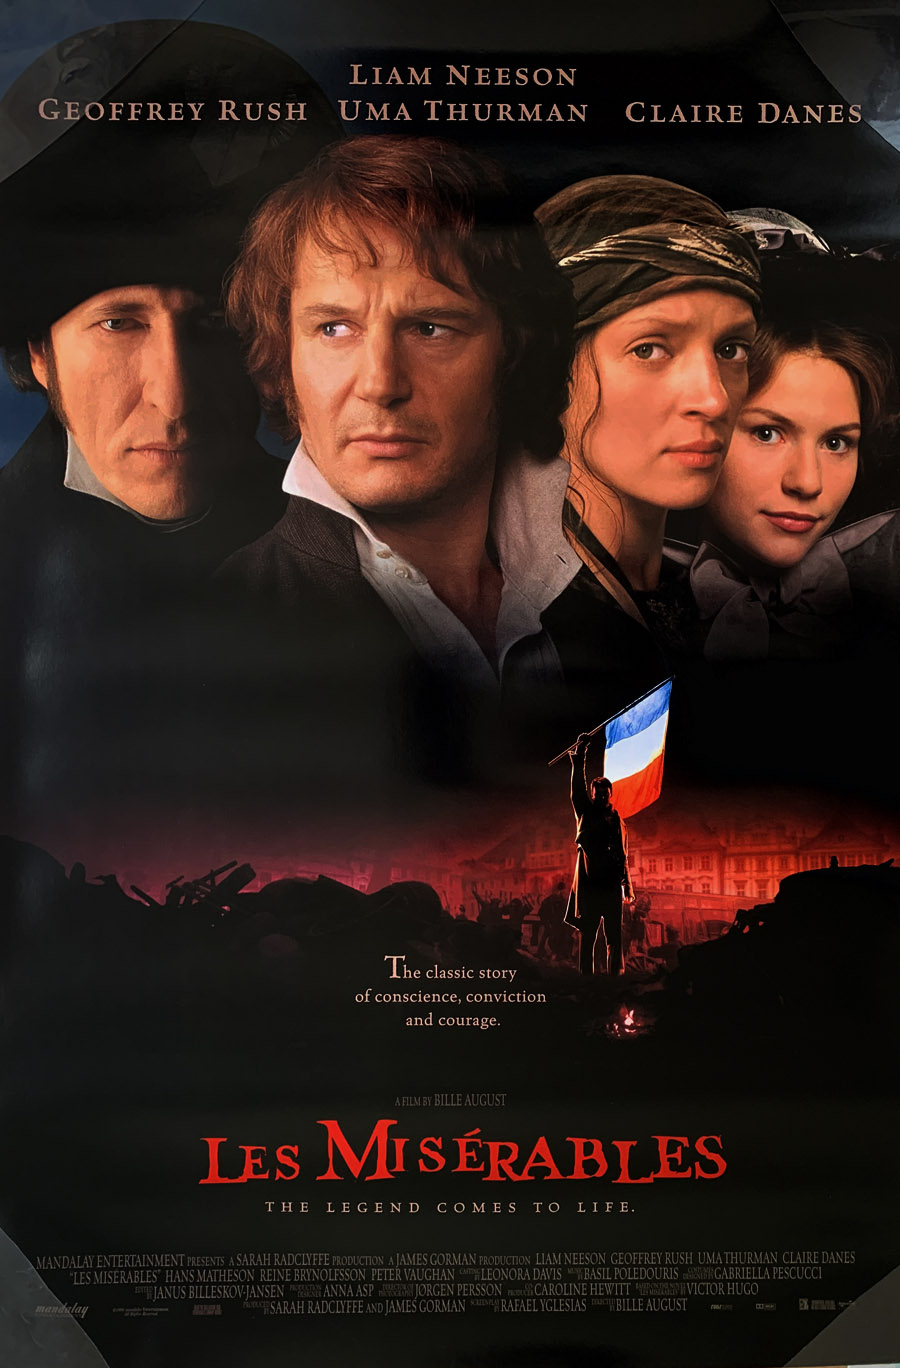
\includegraphics[height=1.5cm, keepaspectratio]{images/movies/les_miserables.png} \\
\hline
\textbf{Név} & MIB & ST & AV & B & SS & LM\\ 
\hline
Sara & $2.20$ & $0.20$ & ? & $-0.80$ & $-0.80$ & $-0.80$\\ 
\hline
Jesper & $0.60$ & $-0.40$ & $0.60$ & ? & $-0.40$ & $-0.40$\\ 
\hline
Therese & $2.33$ & $-0.67$ & $2.33$ & $-0.67$ & $-1.67$ & $-1.67$\\ 
\hline
Helle & $0.40$ & $2.40$ & $0.40$ & ? & $-1.60$ & $-1.60$\\ 
\hline
Pietro & $-0.33$ & $-0.33$ & $-0.33$ & $-1.33$ & $0.67$ & $1.67$\\ 
\hline
Ekaterina & $-1.33$ & $-0.33$ & $-1.33$ & $0.33$ & $1.67$ & $1.67$\\ 
\hline
\end{tabular}
\end{footnotesize}
\end{center}
\end{column}
\end{columns}
\end{frame}

\begin{frame}{Normalizált értékelési tábla}
Az értékelési tábla és az adott felhasználó értékelései szerint felírható a normalizált értékelési tábla. A pozitív értékelések az adott felhasználó átlagos értékelésénél jobbnak számítanak, míg a negatívak rosszabbnak. 
\begin{center}
\begin{tabular}{|c|c|c|c|c|c|c|}
\hline
& 

\includegraphics[height=1.5cm, keepaspectratio]{images/movies/men_in_black.png} &
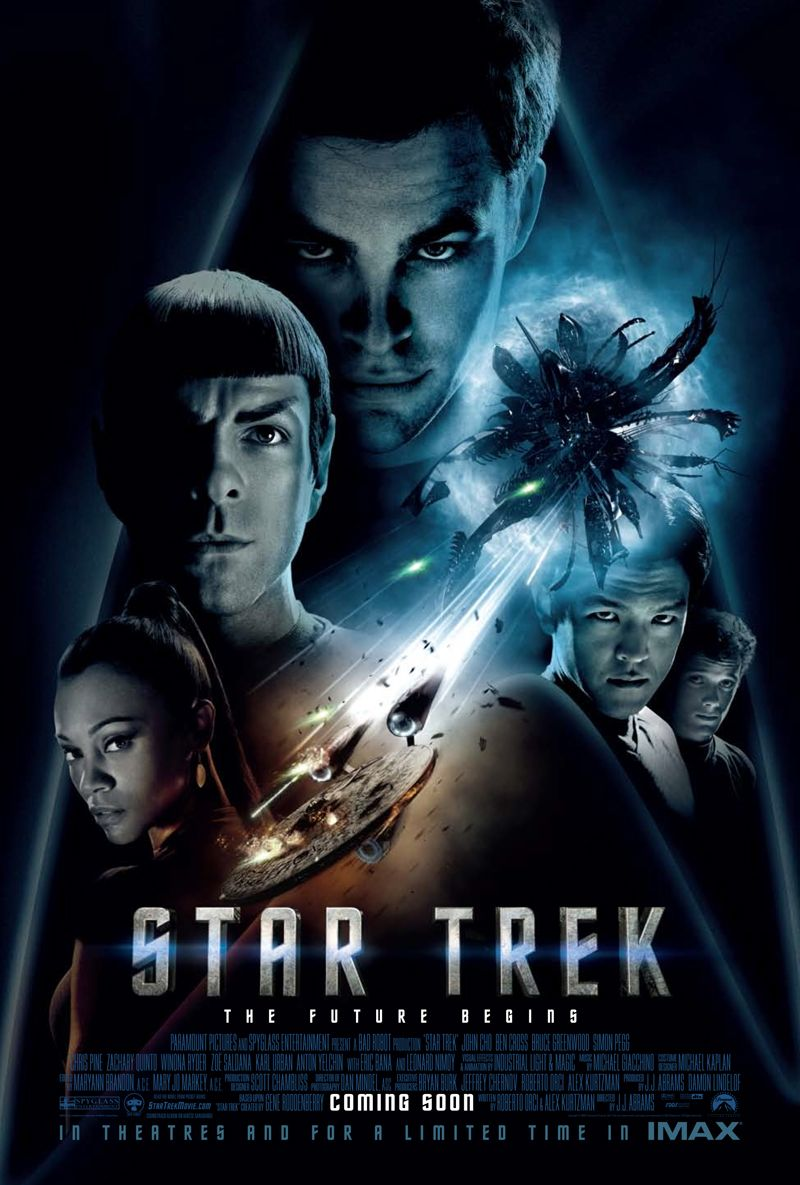
\includegraphics[height=1.5cm, keepaspectratio]{images/movies/star_trek.png} &

\includegraphics[height=1.5cm, keepaspectratio]{images/movies/ace_ventura.png} &

\includegraphics[height=1.5cm, keepaspectratio]{images/movies/braveheart.png} &

\includegraphics[height=1.5cm, keepaspectratio]{images/movies/sense_and_sensibility.png} &
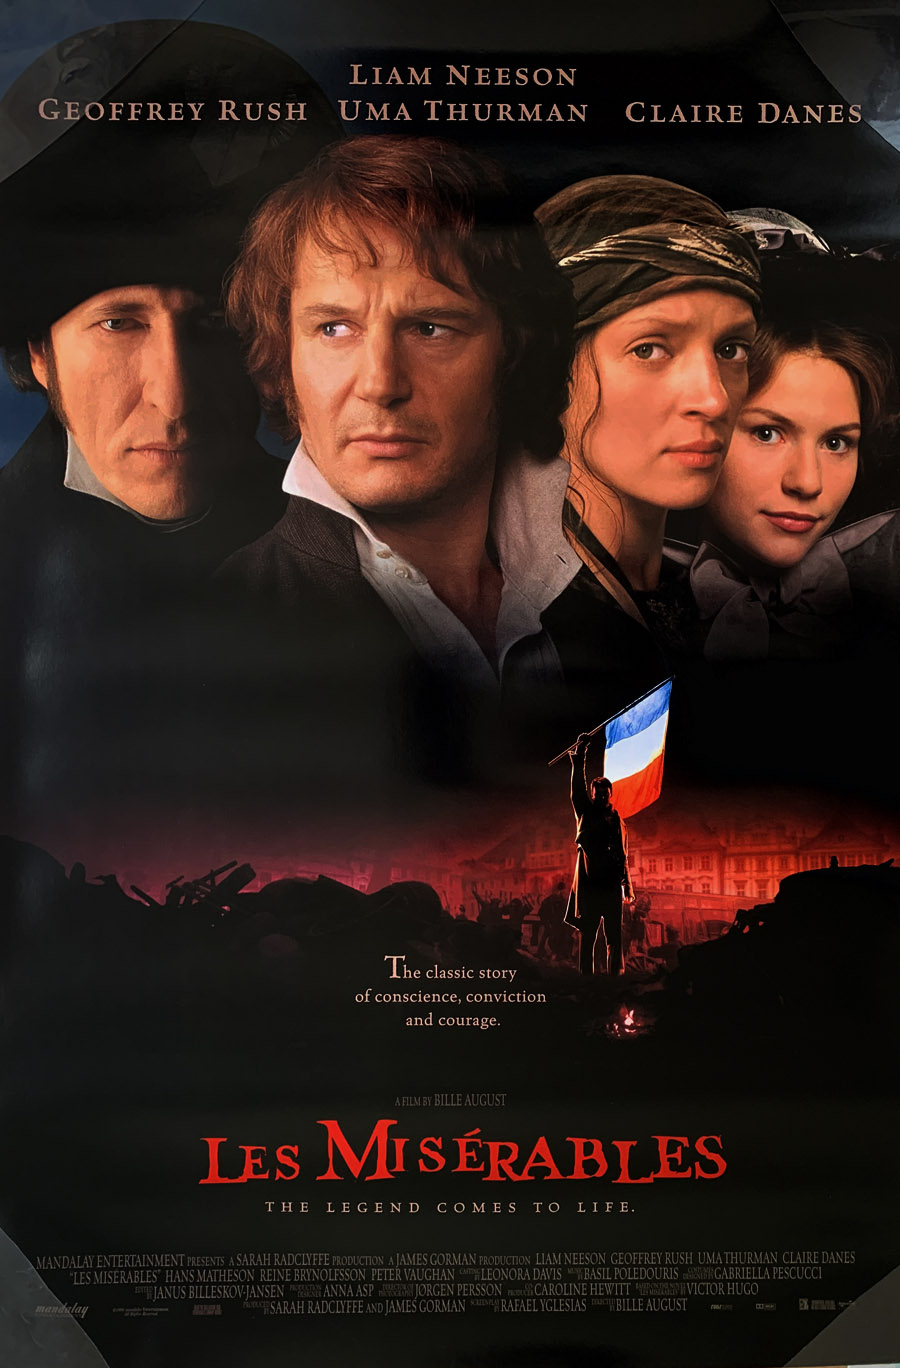
\includegraphics[height=1.5cm, keepaspectratio]{images/movies/les_miserables.png} \\
\hline
\textbf{Név} & MIB & ST & AV & B & SS & LM\\ 
\hline
Sara & $2.20$ & $0.20$ & $?$ & $-0.80$ & $-0.80$ & $-0.80$ \\
\hline
Jesper & $0.60$ & $-0.40$ & $0.60$ & $?$ & $-0.40$ & $-0.40$ \\
\hline
Therese & $2.33$ & $-0.67$ & $2.33$ & $-0.67$ & $-1.67$ & $-1.67$ \\
\hline
Helle & $0.40$ & $2.40$ & $0.40$ & $?$ & $-1.60$ & $-1.60$ \\
\hline
Pietro & $-0.33$ & $-0.33$ & $-0.33$ & $-1.33$ & $0.67$ & $1.67$ \\
\hline
Ekaterina & $-1.33$ & $-0.33$ & $-1.33$ & $-0.33$ & $1.67$ & $1.67$ \\
\hline
\end{tabular}
\end{center}
\end{frame}

\begin{frame}{Korreláció számítása}
A normalizált értékelésekre korrelációs együtthatót számítva előáll a normalizált termék-termék korrelációs mátrixot. Az 1 érték jelenti a tökéletes hasonlóságot, -1 érték a tökéletes különbözőséget, 0 pedig a közömbös kapcsolatot. 
\begin{center}
\begin{tabular}{|c|c|c|c|c|c|c|}
\hline
& 

\includegraphics[height=1.5cm, keepaspectratio]{images/movies/men_in_black.png} &
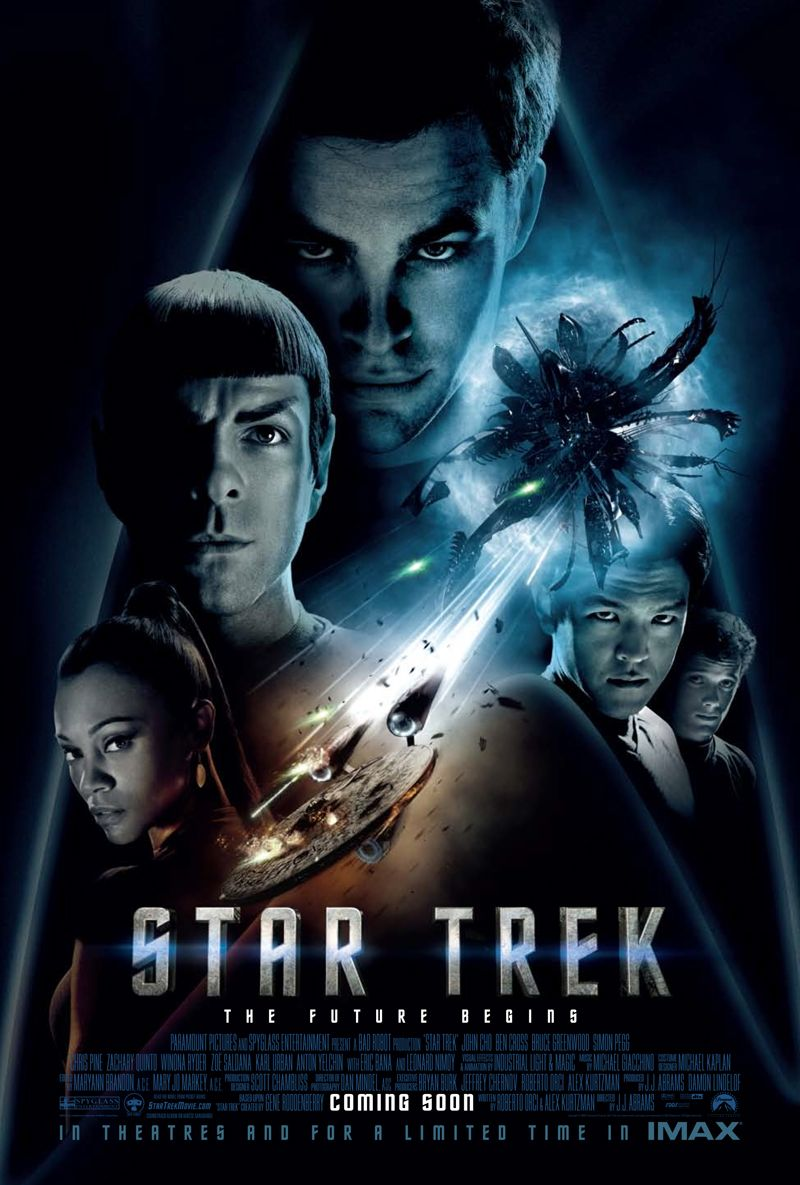
\includegraphics[height=1.5cm, keepaspectratio]{images/movies/star_trek.png} &

\includegraphics[height=1.5cm, keepaspectratio]{images/movies/ace_ventura.png} &

\includegraphics[height=1.5cm, keepaspectratio]{images/movies/braveheart.png} &

\includegraphics[height=1.5cm, keepaspectratio]{images/movies/sense_and_sensibility.png} &
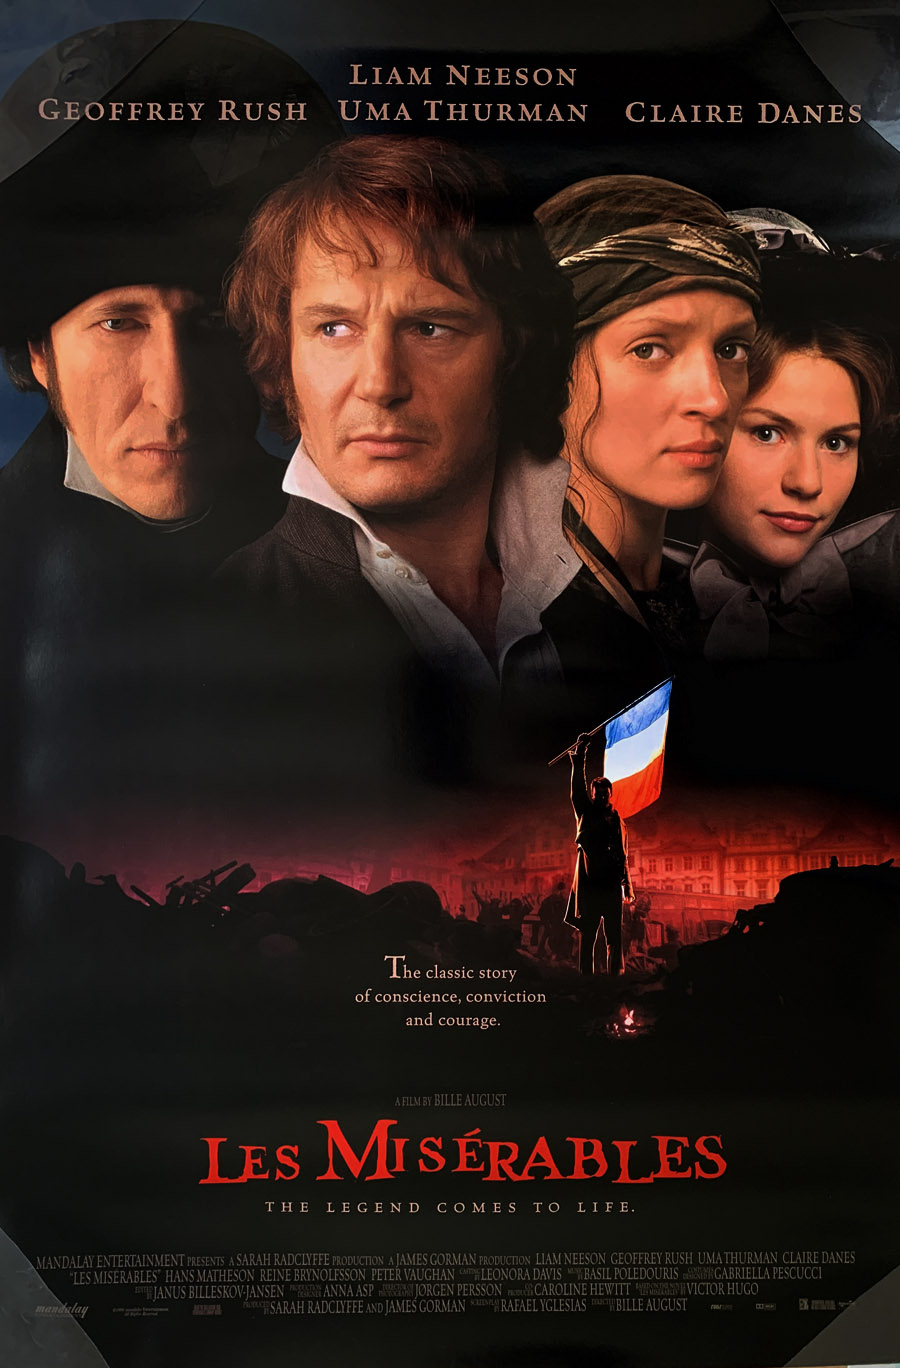
\includegraphics[height=1.5cm, keepaspectratio]{images/movies/les_miserables.png} \\
\hline
\textbf{Név} & MIB & ST & AV & B & SS & LM\\ 
\hline
MIB & $1$ & $0.63$ & $1$ & $-0.21$ & $0.88$ & $-0.83$ \\
\hline
ST  & $0.63$ & $1$ & $0.35$ & $-0.47$ & $-0.64$ & $-0.62$ \\
\hline
AV  & $1$ & $0.35$ & $1$ & $0.01$ & $-0.89$ & $-0.83$ \\
\hline
B   & $-0.21$ & $-0.47$ & $0.01$ & $1$ & $-0.23$ & $-0.32$ \\
\hline
SS  & $0.88$ & $-0.64$ & $-0.89$ & $-0.23$ & $1$ & $0.96$ \\
\hline
LM  & $-0.83$ & $-0.62$ & $-0.83$ & $-0.32$ & $0.96$ & $1$ \\
\hline
\end{tabular}
\end{center}
\end{frame}

\section{Tartalom alapú rendszerek}

\begin{frame}
\tableofcontents[currentsection]
\end{frame}

\begin{frame}{Tartalom alapú rendszerek}
\begin{columns}
\begin{column}{.5\textwidth}
A kollaboratív szűrőkkel ellentétben a tartalom alapú szűrőknek nincs szükségi információra múltbeli vásárlásokról és információról. Ehelyett a javaslatokat a felhasználók profiljai és a termékek metaadatai alapján állítják össze.\par\smallskip
A tartalom alapú rendszerek viszont nem használják ki a közösség adta lehetőségeket.
\end{column}
\begin{column}{.5\textwidth}

\end{column}
\end{columns}
\end{frame}

\end{document}























